\subsection{Estimate High-fidelity 3D Human Body Models from a Single Image using Deep Learning}

\begin{frame}
    \frametitle{Estimate High-fidelity 3D Human Body Models from a Single Image using Deep Learning}
    \begin{block}{What}
        \small
        An end-to-end framework that can estimate 3D mesh of the human body from a single RGB image.    
    \end{block}
    \begin{figure}
        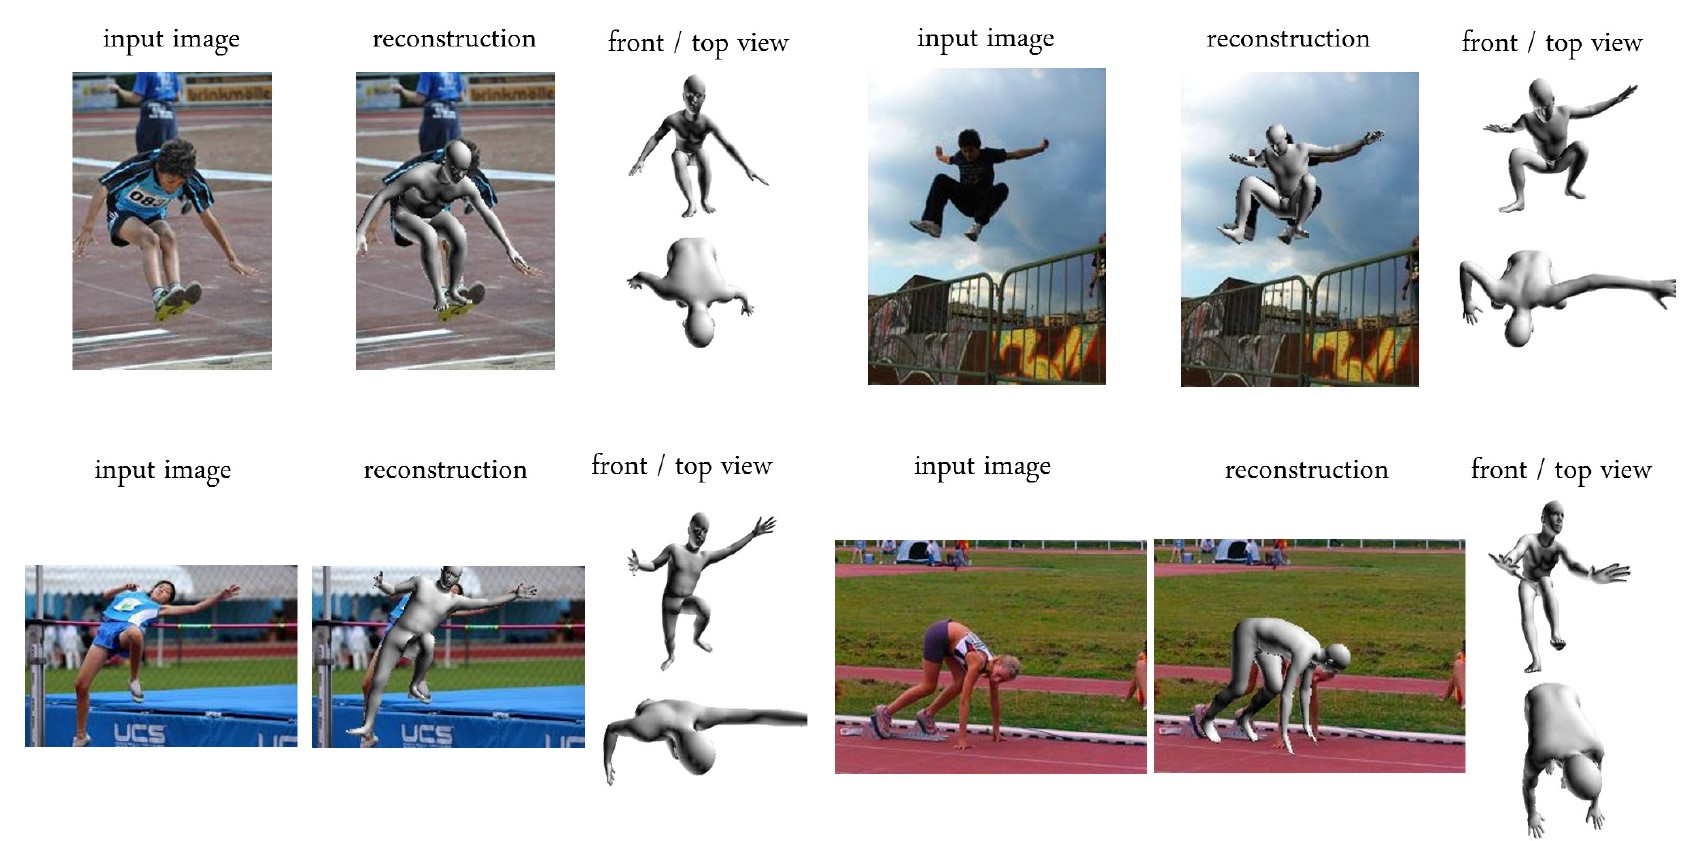
\includegraphics[width=0.8\linewidth]{./img/results_HMR.jpg}
    \end{figure}
\end{frame}

\begin{frame}
    \frametitle{Estimate High-fidelity 3D Human Body Models from a Single Image using Deep Learning}

    \begin{block}{Why}
        \begin{itemize}
        \small
        \item Many existing methods only estimate 3D joints or skeletons (pose), but ignore the 3D shape;
        \item Many existing methods have multiple stages leading to a loss of information;
        \item The lack of in-the-wile images with ground truth 3D annotations.
        \end{itemize}    
    \end{block}

    \begin{block}{How}
        \begin{itemize}
        \small
        \item Apply a skinned multi-person linear (SMPL) model \cite{bogo2016keep} to catch up both 3D pose and shape;
        \item Develop an end-to-end network;
        \item Train the network with a Generative Adversarial Network (GAN) \cite{mirza2014conditional};
        \item Train the network in an iterative error feedback manner (IEF) \cite{carreira2016human}.
        \end{itemize}    
    \end{block}
\end{frame}

\begin{frame}
    \frametitle{Estimate High-fidelity 3D Human Body Models from a Single Image using Deep Learning}
    \begin{itemize}
        \item Framework
        \begin{figure}
            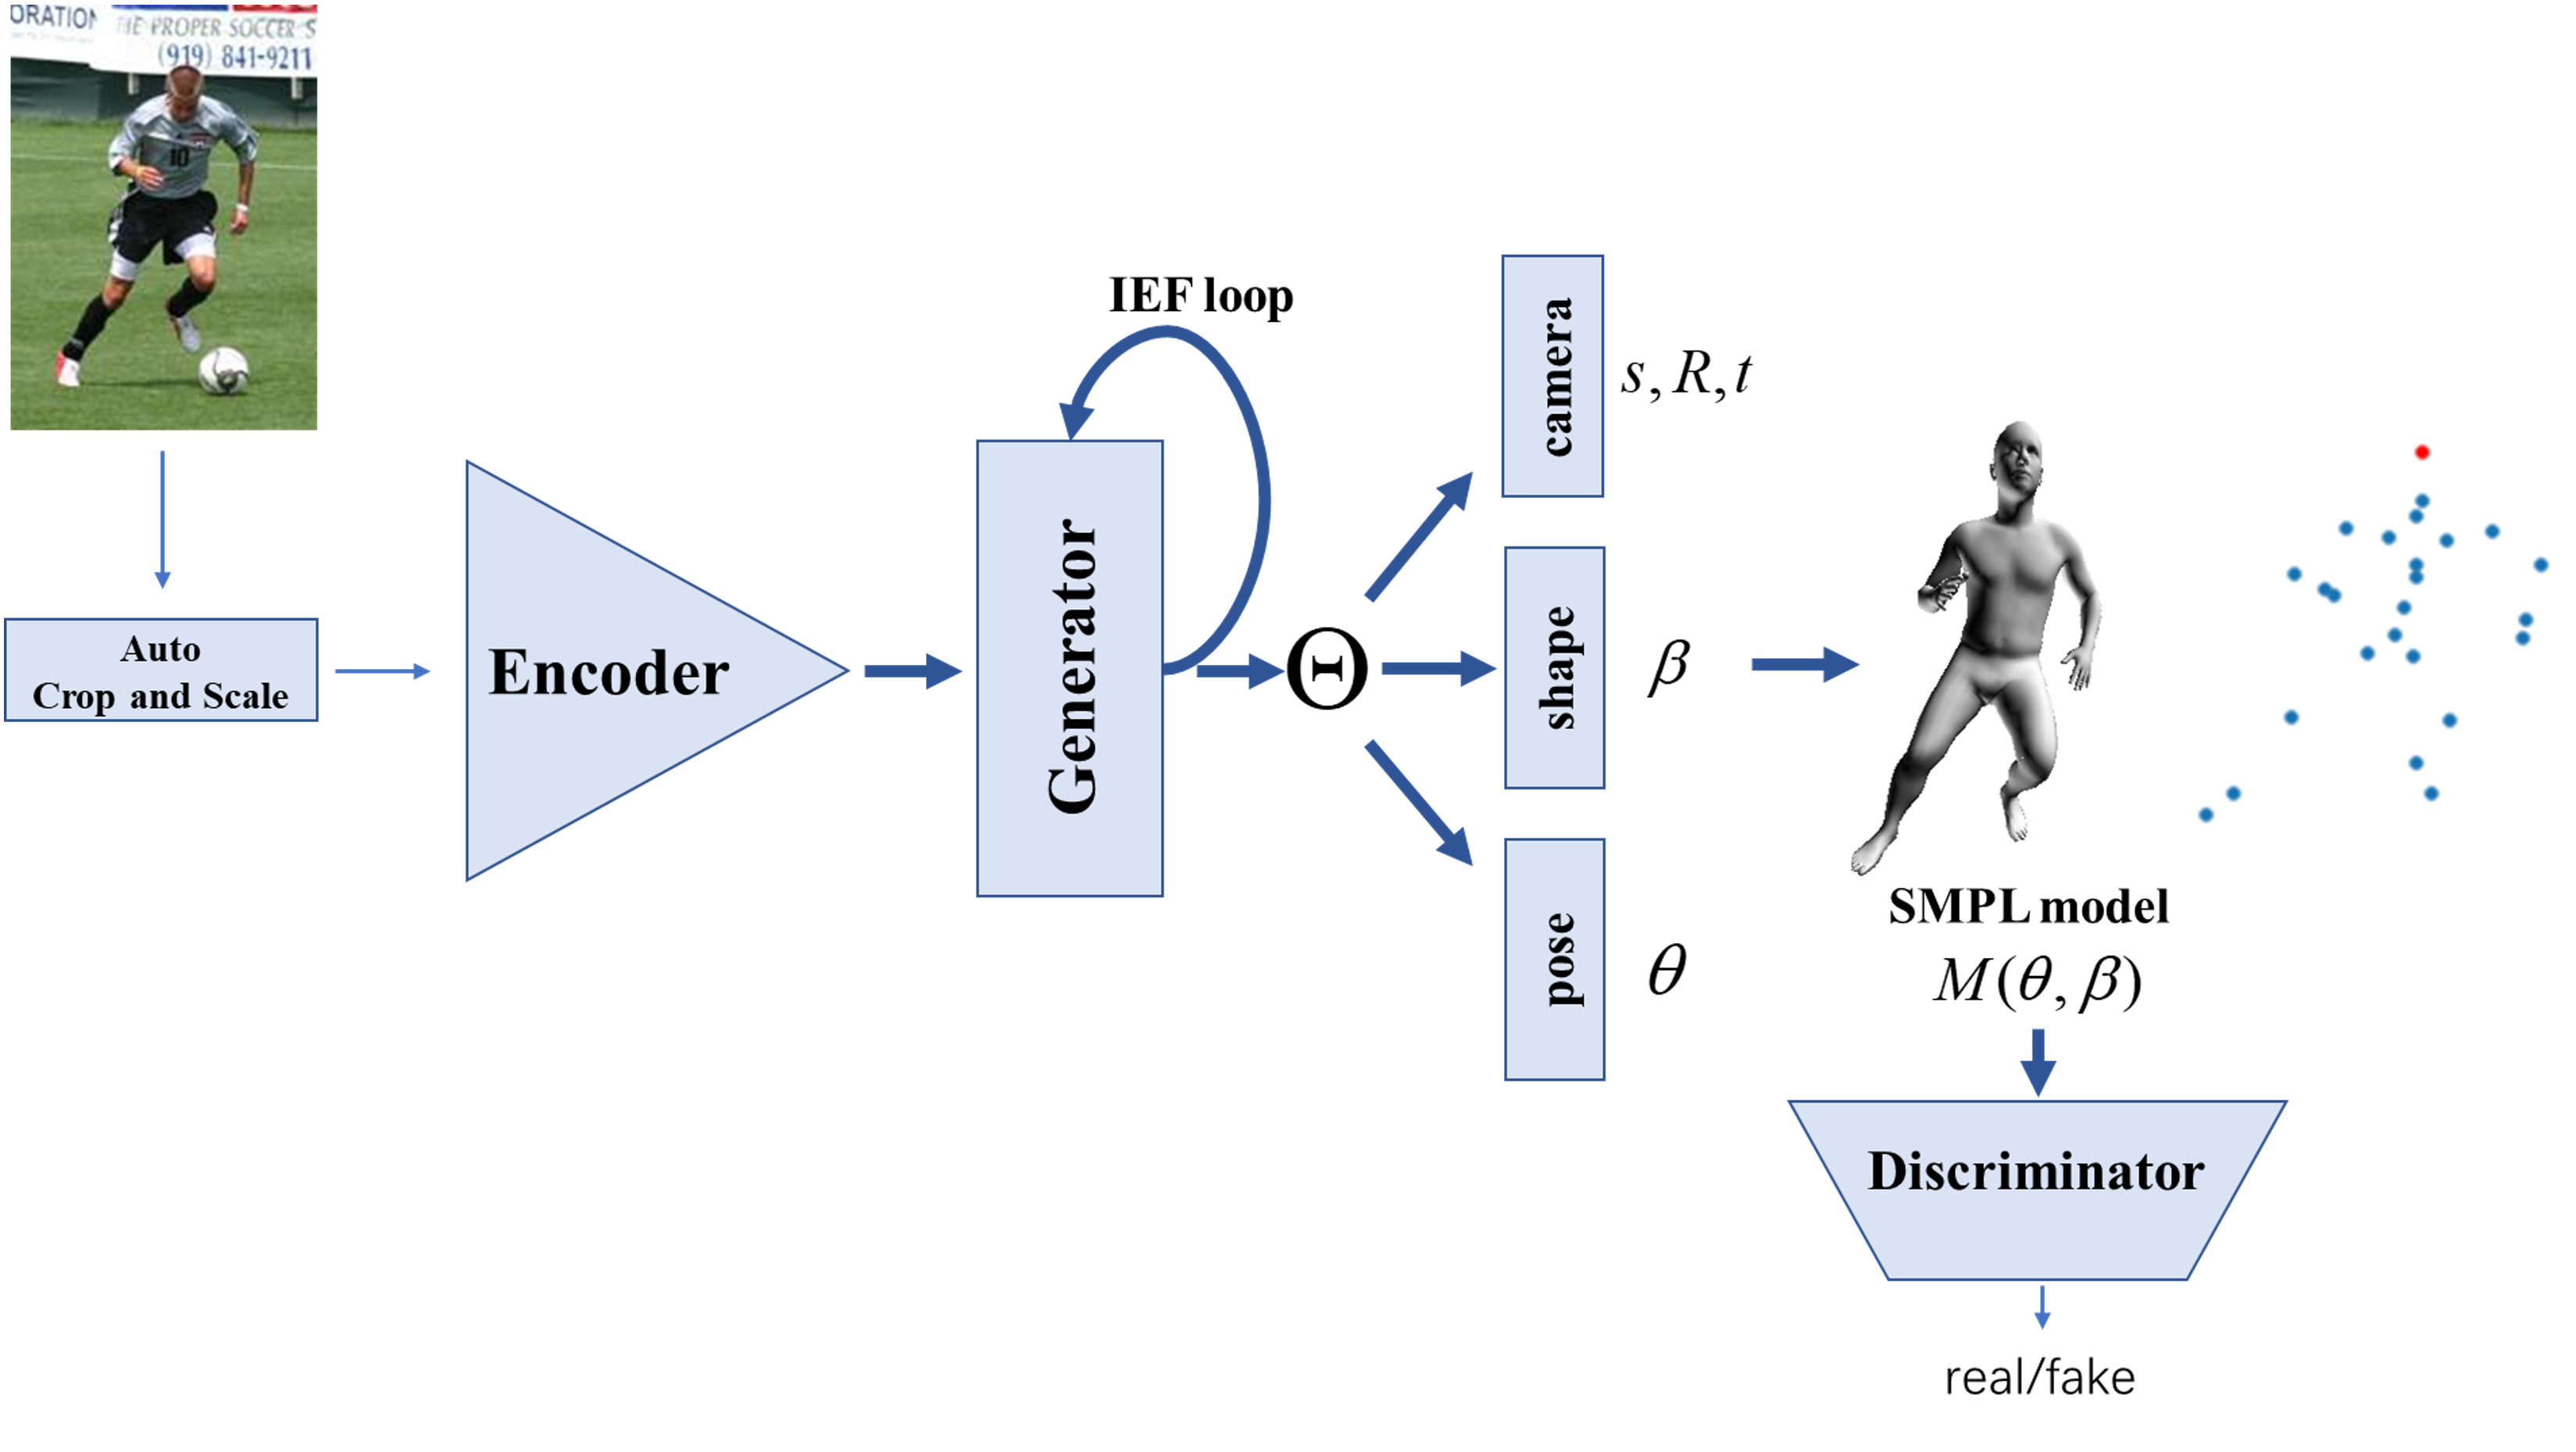
\includegraphics[width=1.0\linewidth]{./img/framework_HMR.png}
        \end{figure}
    \end{itemize}
\end{frame}

\begin{frame}
    \frametitle{Estimate High-fidelity 3D Human Body Models from a Single Image using Deep Learning}
    \begin{block}{Conclusion}
        \begin{itemize}
        \small
        \item With GAN, the overall network can be trained without the in-the-wild images with ground truth 3D annotations, but can still perform well on in-the-wild image.
        \item The training of this network only needs the in-the-wild images with ground truth 2D annotations. Thus, it is easier to improve in the future.       
        \item As the network is end-to-end, the 3D model can be generated fast or even in real time.
        \end{itemize}    
    \end{block}
    % \begin{block}{Limitation}
    %     \begin{itemize}
    %     \small
    %     \item Training GAN requires high computing capability and may cost large resources.
    %     \item As the in-the-wild images with 3D annotations are not used, there is a loss of performance in terms of mean square error.
    %     \end{itemize}    
    % \end{block}
\end{frame}
